\section{Augmentations}\label{section:augmentation}

To simulate real-world scenarios when evaluating attribution methods on datasets, this work uses the multiple augmentations technique. All described augmentations happen only when the calculation of the SSIM metric is done and never influences the results of the \textit{Infidelity} and the \textit{Sensitivity} measures. 

\begin{wrapfigure}{l}{0.45\textwidth}
  \setlength{\belowcaptionskip}{-62pt}
  \centering
  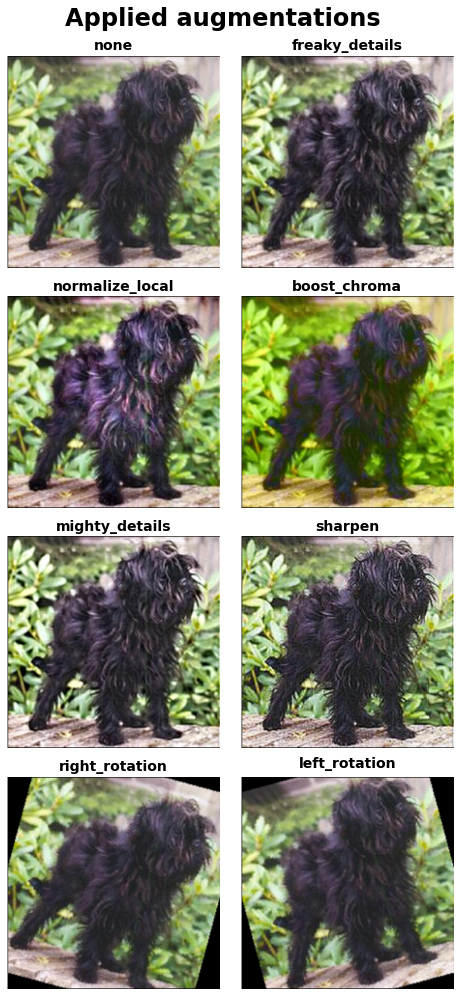
\includegraphics[width=0.40\textwidth]{experiments/aug/augmentations_example.png}
  \caption{Examples  of  real-world augmentations applied on the input image. Image source: \textit{Stanford Dogs} \cite{stanford-dogs}}\label{fig:augmentation-example}
\end{wrapfigure}\leavevmode

\subsection*{Rotation}\label{section:rotations}

This type of augmentation is one of the simplest augmentations we can apply to any image. It uses the rotation matrix\footnote{Rotation matrix is defined as ${\displaystyle R(\theta )={\begin{bmatrix}\cos \theta &-\sin \theta \\\sin \theta &\cos \theta \\\end{bmatrix}}}$ for a two-dimensional vector, where $\theta$ is an angle we want to rotate} to rotate the position of every pixel and fills the empty space with black pixels. This work is using four rotations \textit{\{$-30^{\circ}$ ,$-15^{\circ}$ ,$15^{\circ}$ ,$30^{\circ}$\}} degrees. Because rotation influences the position of the object on the image, when calculating the SSIM value between two attributions, the same rotation is applied to the attribution of the original image. The result of the applied rotation of $15^{\circ}$ and $-15^{\circ}$ can be seen in Figure \ref{fig:augmentation-example} (bottom row).

\subsection*{Freaky Details}

Freaky details filter \cite{freaky_details} is a method used to enhance details of the input image. It works by creating a copy of the image with inverted color and applying a Bilateral filter \cite{tomasi1998bilateral} to it. After the filter, two images are blended together with a \textit{Vivid Light} mode which blends images base on how "light" is a given pixel. It lightens the pixels that are lighter than 50\% gray color and darkens the pixels that are darker than 50\% gray color. The result of the applied filter can be seen in Figure \ref{fig:augmentation-example} in column 2, row 1. It can be applied iteratively, but for the purpose of experiments, it is only applied once. 

\subsection*{Normalize Local}

Local Normalization filter \cite{normalize_local} is a filter that uses local mean and variance to correct local illumination or shading artifacts. For every pixel at the $(x,y)$ position, we normalize its value:

\begin{equation}
    j_{x,y} = \frac{i_{x,y} - \mu_{loc}(i_{x,y})}{\sigma_{loc}(i_{x,y})}
    \label{eq:local-norm-pixel}
\end{equation}

Where $i_{x,y}$ is a value of the pixel at $(x,y)$ position, $\mu_{loc}$ is a mean value of pixels within a given radius, $\sigma_{loc}$ is a variance of the pixels within a given radius. The radius is a parameter, and in the rest of the experiments, it is always $10$ pixels.

\subsection*{Boost Chromaticity}

Boost Chromaticity filter \cite{boost_chroma} is a filter responsible for changing the "colorfulness" of the pixels. It uses the chromaticity diagram to adjust the chromaticity of the pixels. It usually moves the value of the pixel along with the selected color space to avoid spikes on the chromaticity histogram. In the experiments, the $YCbCr$ color space is used.

\subsection*{Mighty Details}

Mighty details filter \cite{mighty_details} is a filter similar to Freaky details. The main difference is that Mighty details apply smoothing (Gaussian blur) before blending two images.

\subsection*{Sharpen}

Sharpening filter \cite{sharpen} is one of the basic filters available in most image processing software. It uses Gaussian blur to create a blurred version of the original image. A blurred image is then compared with the original image, and if the difference between them is greater than a specific threshold, images are subtracted.